\documentclass[10pt, a4paper, twocolumn]{article} % 10pt font size (11 and 12 also possible), A4 paper (letterpaper for US letter) and two column layout (remove for one column)

%%%%%%%%%%%%%%%%%%%%%%%%%%%%%%%%%%%%%%%%%
% Wenneker Article
% Structure Specification File
% Version 1.0 (28/2/17)
%
% This file originates from:
% http://www.LaTeXTemplates.com
%
% Authors:
% Frits Wenneker
% Vel (vel@LaTeXTemplates.com)
%
% License:
% CC BY-NC-SA 3.0 (http://creativecommons.org/licenses/by-nc-sa/3.0/)
%
%%%%%%%%%%%%%%%%%%%%%%%%%%%%%%%%%%%%%%%%%

%----------------------------------------------------------------------------------------
%	PACKAGES AND OTHER DOCUMENT CONFIGURATIONS
%----------------------------------------------------------------------------------------

\usepackage[spanish]{babel} % Spanish language hyphenation

\usepackage{microtype} % Better typography

\usepackage{color}

\usepackage{colortbl}

\usepackage{amsmath,amsfonts,amsthm} % Math packages for equations

\usepackage[svgnames]{xcolor} % Enabling colors by their 'svgnames'

\usepackage[hang, small, labelfont=bf, up, textfont=it]{caption} % Custom captions under/above tables and figures

\usepackage{booktabs} % Horizontal rules in tables

\usepackage{lastpage} % Used to determine the number of pages in the document (for "Page X of Total")

\usepackage{hyperref}

\usepackage{graphicx} % Required for adding images

% PONER EL PAQUETE DE HIPERVÍNCULOS

\usepackage{enumitem} % Required for customising lists
\setlist{noitemsep} % Remove spacing between bullet/numbered list elements

\usepackage{sectsty} % Enables custom section titles
\allsectionsfont{\usefont{OT1}{phv}{b}{n}} % Change the font of all section commands (Helvetica)


\usepackage{listings}
%----------------------------------------------------------------------------------------
%	DEFINITIONS
%----------------------------------------------------------------------------------------

\graphicspath{
    {.} % document root dir
    {images/}
}

%----------------------------------------------------------------------------------------
%	XML LISTINGS
%----------------------------------------------------------------------------------------
\definecolor{dkgreen}{rgb}{0,0.6,0}
\definecolor{gray}{rgb}{0.5,0.5,0.5}
\definecolor{mauve}{rgb}{0.58,0,0.82}
\definecolor{gray}{rgb}{0.4,0.4,0.4}
\definecolor{darkblue}{rgb}{0.0,0.0,0.6}
\definecolor{lightblue}{rgb}{0.0,0.0,0.9}
\definecolor{cyan}{rgb}{0.0,0.6,0.6}
\definecolor{darkred}{rgb}{0.6,0.0,0.0}
%	TCL COLORS

\definecolor{TCLmauve}{rgb}{0.58,0,0.82}
\definecolor{TCLblue}{rgb}{0.1176,0.6039,0.8784}
\definecolor{TCLdkgreen}{rgb}{0,0.6,0}

\lstset{
  basicstyle=\ttfamily\footnotesize,
  columns=fullflexible,
  showstringspaces=false,
  numbers=left,                   % where to put the line-numbers
  numberstyle=\tiny\color{gray},  % the style that is used for the line-numbers
  stepnumber=1,
  numbersep=5pt,                  % how far the line-numbers are from the code
  backgroundcolor=\color{white},      % choose the background color. You must add \usepackage{color}
  showspaces=false,               % show spaces adding particular underscores
  showstringspaces=false,         % underline spaces within strings
  showtabs=false,                 % show tabs within strings adding particular underscores
  frame=none,                   % adds a frame around the code
  rulecolor=\color{black},        % if not set, the frame-color may be changed on line-breaks within not-black text (e.g. commens (green here))
  tabsize=2,                      % sets default tabsize to 2 spaces
  captionpos=b,                   % sets the caption-position to bottom
  breaklines=true,                % sets automatic line breaking
  breakatwhitespace=false,        % sets if automatic breaks should only happen at whitespace
  title=\lstname,                   % show the filename of files included with \lstinputlisting;
                                  % also try caption instead of title  
  commentstyle=\color{gray}\upshape
}

\lstdefinelanguage{XML}
{
  morestring=[s][\color{dkgreen}]{'}{'},
  morestring=[s][\color{mauve}]{"}{"},
  morestring=[s][\color{black}]{>}{<},
  morecomment=[s]{<?}{?>},
  morecomment=[s][\color{dkgreen}]{<!--}{-->},
  stringstyle=\color{black},
  identifierstyle=\color{lightblue},
  keywordstyle=\color{red},
  morekeywords={tipo,version,n,pn,icon,help,actualize_tree,v}% list your attributes here
}

\lstdefinelanguage{tcl}
{
  morestring=[s][\color{TCLmauve}]{"}{"},
  morecomment=[l][\color{TCLblue}]{\#},
  morekeywords={set,variable,list,expr,lindex,puts},
  keywordstyle=\color{red},
  stringstyle=\color{TCLdkgreen},
  %morekeywords={tipo}% list your attributes here
}

%----------------------------------------------------------------------------------------
%	MARGINS AND SPACING
%----------------------------------------------------------------------------------------

\usepackage{geometry} % Required for adjusting page dimensions

\geometry{
	top=1cm, % Top margin
	bottom=1.5cm, % Bottom margin
	left=2cm, % Left margin
	right=2cm, % Right margin
	includehead, % Include space for a header
	includefoot, % Include space for a footer
	%showframe, % Uncomment to show how the type block is set on the page
}




\setlength{\columnsep}{7mm} % Column separation width

%----------------------------------------------------------------------------------------
%	FONTS
%----------------------------------------------------------------------------------------

\usepackage[T1]{fontenc} % Output font encoding for international characters
\usepackage[utf8]{inputenc} % Required for inputting international characters

\usepackage{XCharter} % Use the XCharter font

%----------------------------------------------------------------------------------------
%	HEADERS AND FOOTERS
%----------------------------------------------------------------------------------------

\usepackage{fancyhdr} % Needed to define custom headers/footers
\pagestyle{fancy} % Enables the custom headers/footers

\renewcommand{\headrulewidth}{0.0pt} % No header rule
\renewcommand{\footrulewidth}{0.4pt} % Thin footer rule

\renewcommand{\sectionmark}[1]{\markboth{#1}{}} % Removes the section number from the header when \leftmark is used

%\nouppercase\leftmark % Add this to one of the lines below if you want a section title in the header/footer

% Headers
\lhead{} % Left header
\chead{\textit{\thetitle}} % Center header - currently printing the article title
\rhead{} % Right header

% Footers
\lfoot{} % Left footer
\cfoot{} % Center footer
\rfoot{\footnotesize Page \thepage\ of \pageref{LastPage}} % Right footer, "Page 1 of 2"

\fancypagestyle{firstpage}{ % Page style for the first page with the title
	\fancyhf{}
	\renewcommand{\footrulewidth}{0pt} % Suppress footer rule
}

%----------------------------------------------------------------------------------------
%	TITLE SECTION
%----------------------------------------------------------------------------------------

\definecolor{BlueGiD}{cmyk}{0.77,0.17,0.15,0.0}
\definecolor{GrayGiD}{cmyk}{0.82,0.69,0.55,0.59}

\newcommand{\authorstyle}[1]{{\large\usefont{OT1}{phv}{b}{n}\color{GrayGiD}#1}} % Authors style (Helvetica)

\newcommand{\institution}[1]{{\footnotesize\usefont{OT1}{phv}{m}{sl}\color{Black}#1}} % Institutions style (Helvetica)

\usepackage{titling} % Allows custom title configuration

\newcommand{\HorRule}{\color{BlueGiD}\rule{\linewidth}{1pt}} % Defines the gold horizontal rule around the title

\pretitle{
	\vspace{-30pt} % Move the entire title section up
	\HorRule\vspace{10pt} % Horizontal rule before the title
	\fontsize{32}{36}\usefont{OT1}{phv}{b}{n}\selectfont % Helvetica
	\color{GrayGiD} % Text colour for the title and author(s)
}

\posttitle{\par\vskip 15pt} % Whitespace under the title

\preauthor{} % Anything that will appear before \author is printed

\postauthor{ % Anything that will appear after \author is printed
	\vspace{10pt} % Space before the rule
	\par\HorRule % Horizontal rule after the title
	\vspace{20pt} % Space after the title section
}

%----------------------------------------------------------------------------------------
%	ABSTRACT
%----------------------------------------------------------------------------------------

\usepackage{lettrine} % Package to accentuate the first letter of the text (lettrine)
\usepackage{fix-cm}	% Fixes the height of the lettrine

\newcommand{\initial}[1]{ % Defines the command and style for the lettrine
	\lettrine[lines=3,findent=4pt,nindent=0pt]{% Lettrine takes up 3 lines, the text to the right of it is indented 4pt and further indenting of lines 2+ is stopped
		\color{BlueGiD}% Lettrine colour
		{#1}% The letter
	}{}%
}

\usepackage{xstring} % Required for string manipulation

\newcommand{\lettrineabstract}[1]{
	\StrLeft{#1}{1}[\firstletter] % Capture the first letter of the abstract for the lettrine
	\initial{\firstletter}\textbf{\StrGobbleLeft{#1}{1}} % Print the abstract with the first letter as a lettrine and the rest in bold
}

%----------------------------------------------------------------------------------------
%	BIBLIOGRAPHY
%----------------------------------------------------------------------------------------

\usepackage[backend=bibtex,style=authoryear,natbib=true]{biblatex} % Use the bibtex backend with the authoryear citation style (which resembles APA)

\addbibresource{example.bib} % The filename of the bibliography

\usepackage[autostyle=true]{csquotes} % Required to generate language-dependent quotes in the bibliography
 % Specifies the document structure and loads requires packages

%----------------------------------------------------------------------------------------
%	ARTICLE INFORMATION
%----------------------------------------------------------------------------------------

\title{Primer acercamiento al desarrollo de Problem Types en GiD} % The article title

\author{
	\authorstyle{Luis G. Yáñez Rodríguez\textsuperscript{1}} % Authors
	\newline\newline % Space before instittions
	\textsuperscript{1}\institution{Universidad de Guanajuato, Guanajuato, México}\\ % Institution 1
}

% Example of a one line author/institution relationship
%\author{\newauthor{John Marston} \newinstitution{Universidad Nacional Autónoma de México, Mexico City, Mexico}}

\date{Febrero, 2018} % Add a date here if you would like one to appear underneath the title block, use \today for the current date, leave empty for no date

%----------------------------------------------------------------------------------------

\begin{document}

\maketitle % Print the title

\thispagestyle{firstpage} % Apply the page style for the first page (no headers and footers)

%----------------------------------------------------------------------------------------
%	ABSTRACT
%----------------------------------------------------------------------------------------

\lettrineabstract{Sin duda alguna, los modelos computacionales nos han permitido entender el mundo que nos rodea. Ya sea para explicar de una mejor manera un fenómeno o para poder predecirlo. Parte del éxito de estas soluciones tiene que ver con que estas se apoyan de elementos gráficos para la presentación de resultados, en resumen tener algo más o menos ``tangible'', ya que todas las soluciones que en estos métodos se encuentran se resumen en ceros y unos. Existen muchos softwares que ayudan en el pre y post proceso de un método computacional, pero entre ellos destaca uno en particular llamado GiD, The personal pre and post processor, desarrollado por el CIMNE, el cual que permite una amplia adaptación al problema en cuestión y customización de los procesos del modelado matemático.}

\section{Justificación}

Cuando se usa GiD para un análisis en particular, es necesario establecer los parámetros a los que el modelo estará sujeto (preproceso). En esta parte se definen parámetros como, condiciones, materiales, datos generales, sistema de unidades, símbolos y el formato del archivo de salida para el solver\footnote{Conjunto de rutinas de programación para resolver un problema numérico en específico.}. Gracias a la característica de adaptación de \textit{GiD}, los desarrolladores del software crearon una colección de archivos llamada \textbf{Problem Type} que definen los parámetros anteriores. Actualmente la documentación disponible acerca del desarrollo de problem types se encuentra en el idioma inglés, lo cual puede ser una limitante para aquellos que quieran incursionar en el desarrollo de las herramientas. 

\begin{figure}[hbt!]\centering
	
\includegraphics[width=0.2\textwidth]{logoGiD.PNG}
	\caption{Logo de GiD.}
\end{figure}

\subsection{Objetivo}

Este documento pretende ser un ``primer acercamiento'' a los problem types para aquellas personas de habla hispana en donde tal vez no encuentren toda la información, pero sí puedan tener un apoyo.

\subsection{Aplicación}

Cabe señalar que este material será sólo un apoyo para la \textit{customización}, no es un manual de usuario de GiD, este se puede encontrar en \textcolor{BlueGiD}{\underline{\url{www.gidhome.com/support/gid-manuals/}}} . En caso de tener dudas muy puntuales el material de apoyo es muy amplio y siempre se puede consultar el \textit{Manual de Customización} o directamente en los foros de ayuda en donde los desarrolladores de GiD ayudarán, el link es \textcolor{BlueGiD}{\underline{\url{www.gidhome.com/forum/}}}.

\section{Primeros pasos}

¿Qué es lo que hace interesante GiD?. La respuesta es la \textbf{programación}, GiD está escrito para que sea de propósito general, de manera que los usuarios pueden crear sus propios solvers y manipular la información que sale y entra en él. Para explicar lo anterior, se tiene el siguiente diagrama:

\begin{figure}[hbt!]\centering
	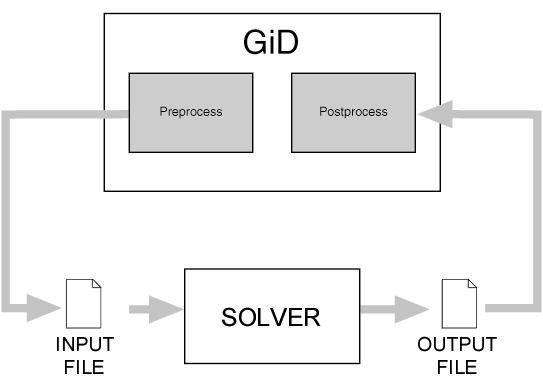
\includegraphics[width=0.35\textwidth]{etapasGiD.PNG}
	\caption{Diagrama de los procesos que realiza un Problem Type.}
	\label{fig:diagramaProcesos}
\end{figure}

La manera como se escribían anteriormente los \textit{problem types} era un poco rudimentaria, de manera que con unas cuantas instrucciones se desplegaban ventanas para la entrada de datos, imposibilitando personalizar estas ventanas.

Desde la versión 13 de GiD, se ha implementado una nueva versión de problem type (basado en la librería CustoLIB), aunque el sistema ``clásico'' sigue siendo soportado por GiD. Esta nueva versión usa un único archivo \texttt{.spd} para describir las propiedades generales, materiales, condiciones y unidades (como un árbol en la sintaxis de \textbf{XML}\footnote{eXtensible Markup Language.}). Toda esta información se muestra en una ``vista de árbol'' y los materiales y condiciones son asociados en grupos de entidades.

Toda esta información es leída y procesada mediante el lenguaje de programación \textbf{TCL}, lenguaje orientado a objetos que permitirá crear interfaces gráficas de usuario (GUI) y darle un mejor aspecto a los problem types.

La combinación de TCL y XML, definirá el rumbo que el usuario le de a su problem type, es por ello que es importante leer y aprender de estas dos herramientos. Una buena guía para TCL se puede encontrar en: \textcolor{BlueGiD}{\underline{\url{www.tcl.tk/doc/}}}, y para XML en: \textcolor{BlueGiD}{\underline{\url{www.w3schools.com/xml/}}}.

\subsection{El sistema del problem type}

Como ya se dijo, un problem type es una colección de utilidades, las cuales permiten al usuario interactuar fácilmente con ellos mediante una GUI y facilita la definición e introducción de todos los datos necesarios para abordar un cálculo en particular. Para preparar los tos para un programa de análisis específicos, es necesario personalizarlo primero. La personalización se define en GiD por medio de un problem type.

El nuevo sistema para la creación de un problem type agrega algunas capacidades adicionales comparado con el sistema clásico:

\begin{itemize}
	\item Aprovecha las características de formato de XML y su estructura jerarquizada. Almacena información eficientemente. Los elementos en un documento XML forman una estructura de árbol que ``comienza en la raíz y se ramifica en las hojas'' con diferentes relaciones entre los elementos anidados.
	\item Facilita la creación automática de \textit{ventanas estandarizadas} en el árbol de datos (\textit{data tree}) para introducir datos.
	\item Permite acoplar entidades con propiedades idénticas en grupos.
	\item Permite aplicar eficientemente propiedades geométricas y condiciones de contorno en grupos para editar sus propiedades fácilmente.
\end{itemize}

\subsection{Estructura del problem type}

Un problem type se define usando un directorio con su nombre y arreglo de archivos. El directorio con el problem type estará ubicado en el directorio \textbf{problemtypes} en la distribución \textbf{GiD} que se tenga instalado en la computadora, por ejemplo en Windows 




\section{Bibliografía}


%----------------------------------------------------------------------------------------
%	BIBLIOGRAPHY
%----------------------------------------------------------------------------------------

%\printbibliography[title={Bibliography}] % Print the bibliography, section title in curly brackets

%----------------------------------------------------------------------------------------

\end{document}
